\chapter{ASF: A Library for Automated Algorithm Selection}
\label{ch:ch10:asf}

\section{Introduction}

\Gls{ai} algorithms have shown impressive performance, enabling   continuous improvements to the state of the art in solving problems from computer vision~\citep{KriEtAl12,TsiEtAl21}, natural language processing~\citep{Team25}, \gls{sat} solving~\citep{ShaHoo24} and other domains.
However, performance complementarity between algorithms remains in most, if not all cases: no single algorithm dominates over all problem instances.
This is a well-known phenomenon that can be exploited using \textit{automated algorithm selection} (or, in short, algorithm selection; \citealp{Rice76}).


\begin{figure}
  \centering

\begin{tikzpicture}[
    >=Stealth,
    font=\sffamily\small,
%
    asf-internal/.style={draw=green!60!black, thick, fill=green!10, text width=2.4cm, align=center, minimum height=0.55cm, rounded corners=2pt},
%
    sat-box/.style={draw=red!80!black, thick, fill=red!10, text width=2.0cm, align=center, minimum height=0.9cm, rounded corners=2pt},
    sat-out/.style={draw=red!80!black, thick, fill=red!10, text width=2.3cm, align=center, minimum height=0.7cm, rounded corners=2pt},
    automl-box/.style={draw=blue!80!black, thick, fill=blue!10, text width=2.0cm, align=center, minimum height=0.9cm, rounded corners=2pt},
    automl-out/.style={draw=blue!80!black, thick, fill=blue!10, text width=2.3cm, align=center, minimum height=0.7cm, rounded corners=2pt},
    bbo-box/.style={draw=orange!80!black, thick, fill=orange!10, text width=2.0cm, align=center, minimum height=0.9cm, rounded corners=2pt},
    bbo-out/.style={draw=orange!80!black, thick, fill=orange!10, text width=2.3cm, align=center, minimum height=0.7cm, rounded corners=2pt}
]


    \node[bbo-box] (bbo) at (0, 0) {\textbf{\gls{bbo}}\\ \scriptsize Function};
    \node[automl-box] (automl) [above=0.5cm of bbo] {\textbf{\gls{automl}}\\ \scriptsize Dataset};
    \node[sat-box] (sat) [below=0.5cm of bbo] {\textbf{\gls{sat}}\\ \scriptsize Boolean Formula};


    \node[asf-internal] (presel) at (5.0, 0) {\textbf{Pre-selection}};
    \node[asf-internal] (presol) [above=0.12cm of presel] {\textbf{Pre-solving}};
    \node[asf-internal] (sel) [below=0.12cm of presel] {\textbf{Selection}};
    \node[asf-internal] (tune) [below=0.12cm of sel] {\textbf{Tuning}};


    \node[align=center, above=0.3cm of presol] (title) {\large\textbf{\gls{asf}}\\ \footnotesize Domain Independent};


    \begin{scope}[on background layer]
        \node[draw=green!60!black, thick, fill=green!15, rounded corners=6pt, inner sep=6pt, 
              fit=(title) (presol) (tune)] (asf-core) {};
    \end{scope}


    \draw[ultra thick, draw=blue!80!black, ->] (automl.east) -- (asf-core.west |- automl.east) node[midway, above, font=\tiny, text=black!80] {Feature Extraction};
    \draw[ultra thick, draw=orange!80!black, ->] (bbo.east) -- (asf-core.west |- bbo.east) node[midway, above, font=\tiny, text=black!80] {Feature Extraction};
    \draw[ultra thick, draw=red!80!black, ->] (sat.east) -- (asf-core.west |- sat.east) node[midway, above, font=\tiny, text=black!80] {Feature Extraction};


    \node[automl-out, right=1.8cm of asf-core.east |- automl] (out-automl) {\textbf{Accuracy}\\ \scriptsize(\gls{automl})};
    \node[bbo-out, right=1.8cm of asf-core.east |- bbo] (out-bbo) {\textbf{Regret}\\ \scriptsize(\gls{bbo})};
    \node[sat-out, right=1.8cm of asf-core.east |- sat] (out-sat) {\textbf{Running Time}\\ \scriptsize(\gls{sat})};


    \draw[->, ultra thick, draw=red!80!black] (asf-core.east |- out-sat.west) -- (out-sat.west) node[midway, above, font=\tiny, text=black!80] {Assessment};
    \draw[->, ultra thick, draw=blue!80!black] (asf-core.east |- out-automl.west) -- (out-automl.west) node[midway, above, font=\tiny, text=black!80] {Assessment};
    \draw[->, ultra thick, draw=orange!80!black] (asf-core.east |- out-bbo.west) -- (out-bbo.west) node[midway, above, font=\tiny, text=black!80] {Assessment};

\end{tikzpicture}
  \caption[ASF library overview]{Overview of the \gls{asf} library which provides problem-agnostic implementations of algorithm selection methods, which can be used for various domains, such as \gls{automl}, \gls{bbo}, \gls{sat}, and others.

  }
\end{figure}


Traditionally, algorithm selection methods use instance features as input to one or more machine learning models to decide which algorithm is likely to perform best.

Such methods have shown exceptional performance in many sub-fields of \gls{ai}.
For example, in machine learning, algorithm selection has been a cornerstone in hands-free automated machine learning methods (see, e.g., \citealp{FeuEtAl15}), which create a full machine learning pipeline given an input dataset.
Portfolio-based algorithm selectors have also shown exceptional performance for many $\mathcal{NP}$-complete problems. A well-known example is in the \gls{sat} domain, where SATzilla~\citep{XuEtAl08} won multiple \gls{sat} competitions and consistently outperformed single-solver baselines~\citep{XuEtAl12,ShaHoo24}. Additionally, such approaches have been applied for automated planning, where they outperformed state-of-the-art solvers~\citep{ValEtAl14}.

Algorithm selection has also been applied in various other areas of \gls{ai}, such as out-of-distribution generalisation for neural networks~\citep{JiaTen25}, black-box optimisation~\citep{JonEtAl98} and others.



However, no comprehensive library for state-of-the-art algorithm selection methods exists\footnote{We note that the R library LLAMA~\citep{Kotthoff13} implements only a small number of selection methods and does not support full selection pipelines, as further discussed in \cref{sec:ch10:llama}}. This creates several problems.



Firstly, every research area might develop its own methods, unaware of advances in other areas.
Secondly, since every method is implemented for a specific use case, it can be hard to apply it directly in other areas.
Thirdly, the absence of a central framework negatively affects reproducibility and the ability of researchers to fairly compare new methods to existing ones.

To address these challenges, we introduce the algorithm selection framework (\gls{asf}), the first Python library for problem-agnostic algorithm selection.
\Gls{asf} provides instance-feature and performance-matrix based algorithm selectors through a unified, scikit-learn-like \gls{api}, allowing methods developed in one domain to be reused in another.
The framework implements the main components of algorithm selection pipelines, including pre-selection, pre-solving, selection, tuning and evaluation.

To showcase the advantage of using \gls{asf}, we evaluate it in the context of three important use cases in machine learning: 

zero-shot portfolio selection~\citep{OztEtAl22}, out-of-distribution generalisation~\citep{JiaTen25}, and portfolio construction for hyperparameter optimisation~\citep{EggEtAl21}.
Our empirical results demonstrate that well-known algorithm selection methods, made easily accessible through \gls{asf}, can match or surpass domain-specific implementations, sometimes at a fraction of the training cost. Ultimately, \gls{asf} makes it easier to assess performance complementarity that can be exploited using automated algorithm selection, thereby providing a more systematic foundation for empirical claims in \gls{ai}.

The remainder of the paper is structured as follows: we begin by covering the background of algorithm selection and related methods in \cref{sec:ch10:add_background}, continuing with a presentation of \gls{asf} and its components in \cref{sec:ch10:asf_overview}, followed by our empirical results and discussion in \cref{sec:ch10:experiments}, and concluding in \cref{sec:ch10:conclusion}. Additional benchmarks and details are available in the appendix, and we provide the source code for \gls{asf} at \url{https://anonymous.4open.science/r/asf-660A/}.











\subsection{Empirical performance prediction}
A closely related problem to algorithm selection is empirical performance prediction, where given an instance $I\in\mathcal{I}$ and a feature vector $\mathbf{f}\in\mathcal{F}$, the goal is to create an empirical performance model (\gls{epm}) $P_A:\mathcal{F}\rightarrow \mathbb{R}$ that predicts $m(A, I)$ as accurately as possible.
\Glspl{epm} can be used for algorithm selection~\citep{NudEtAl04,XuEtAl08}, algorithm configuration~\citep{HutEtAl11,LinEtAl22b}, explainability~\citep{HutEtAl13}, and data centre scheduling~\citep{LeeEtAl25}.
To model performance, one should account for the distribution of the performance, which can require preprocessing of the labels, such as log-transformation~\citep{HutEtAl14}. However, \gls{epm}-based algorithm selection is often not the practically best approach, essentially because accurately predicting exact performance values is generally a harder task than determining the relative ranking of algorithms.



\section{Overview of ASF}
\label{sec:ch10:asf_overview}
\Gls{asf} is a modular, \emph{problem-agnostic} Python library for algorithm selection.
At its core, the framework expects instance features together with a performance matrix over candidate algorithms and does not assume a specific application domain such as \gls{sat} solving, automated planning, \gls{automl}, or numerical optimisation.
Any problem that can be described through descriptive features and a measurable target metric can be addressed with \gls{asf}.
This design allows non-experts to apply algorithm selection effectively to new problems.
\Gls{asf} follows a scikit-learn-like \gls{api}~\citep{PedEtAl11}, making it easily accessible to machine learning practitioners.


\textbf{Selectors.}
\Gls{asf} implements a wide variety of algorithm selection methods, including multi-class classification~\citep{Kotthoff13}, pairwise classification~\citep{XuEtAl12} and regression~\citep{KerEtAl18}, empirical-performance-model-based selection~\citep{XuEtAl08}, ranking-based methods, neighbourhood-based methods such as ISAC~\citep{KadEtAl10} and SUNNY~\citep{AmaEtAl14}, and ensemble-based approaches~\citep{TorEtAl23}. Additionally, while looking at algorithm selection as a recommendation system is a known technique~\citep{MisSeb17}, \gls{asf} furthermore implements it using the standard LambdaMART~\citep{Burges10} algorithm with XGBoost~\citep{CheGue16}.
A complete list of the selectors implemented in \gls{asf} is provided in \cref{sec:ch10:methods_implemented}.


\textbf{Pre-selection.}
Before fitting the final selector, \gls{asf} can apply \emph{pre-selectors} to reduce a large candidate set to a compact, complementary portfolio.
The library provides marginal-contribution-based~\citep{XuEtAl08}, beam-search~\citep{BacEtAl22}. Additionally, \gls{asf} implements general optimisation algorithms that, to the best of our knowledge, have not been applied to this task yet, such as random-local-search~\citep{HutEtAl11}, a genetic algorithm~\citep{FraBur70}, differential evolution~\citep{PriEtAl05}, and other pre-selection strategies that operate on the performance matrix alone and return a restricted portfolio (see \cref{sec:ch10:methods_implemented} for a full list).

This is particularly useful when many candidate algorithms are available, as removing redundant or weak alternatives improves statistical efficiency, reduces training time, and lowers the chance of severe prediction errors.

\textbf{Pre-solving.}
\Gls{asf} also supports pre-solving schedules for running time scenarios, such as greedy scheduling~\citep{XuEtAl08}, Aspeed~\citep{HooEtAl12} and 3S~\citep{KadEtAl11}.

\textbf{Pipelines.} \gls{asf} supports creating pipelines of components, such as pre-selection, pre-solving, selection, and data preprocessing (for which, any feature preprocessing that follows \textsc{scikit-learn}~\citep{PedEtAl11} conventions is supported) into a single tunable unit.

\textbf{Hyperparameter optimisation.}
Pipelines and selectors can be automatically tuned using SMAC3~\citep{HutEtAl11,LinEtAl22b}, a well known model-based hyperparameter optimisation library, optionally selecting among multiple selector types (similarly to AutoFolio~\citep{LinEtAl15}). \Gls{asf} includes configuration spaces for all implemented methods, in addition to configuration spaces for the underlying machine learning models.


For every method component (selection, pre-selection, etc.), \gls{asf} provides an abstract class responsible for handling data preprocessing and more. For algorithm selection, there exists an additional abstract class responsible for handling the models used by the selectors (if applicable). We provide an example of how to use \gls{asf} for algorithm selection in \cref{sec:ch10:asf_usage_appendix}.




\section{Case studies for algorithm selection in ML}
\label{sec:ch10:experiments}
In this section, we demonstrate the application of \gls{asf} to three machine learning tasks: zero-shot hyperparameter optimisation in deep learning, selection of out-of-distribution generalisation (\gls{ood}) algorithms, and pre-selection of algorithm portfolios of traditional machine learning algorithms. 
Additional experiments on the well-known ASlib~\citep{BisEtAl16} are available in~\cref{sec:ch10:aslib_appendix}.

\subsection{Zero-shot portfolio selection for AutoML}
\label{sec:ch10:zap}


Training deep learning models typically requires substantial computational resources and large training datasets~\citep{SchEtAl20}. A common strategy to mitigate these requirements is fine-tuning, where a pre-trained neural network is adapted to a target task using a relatively limited amount of computation and data.
However, effective fine-tuning depends on the choice of the pre-trained model and on hyperparameter settings (\emph{e.g.}, optimiser and learning rate). 
Because a primary motivation for fine-tuning is to reduce computational cost, exhaustive hyperparameter optimisation is often infeasible in practice.
To address this limitation, \citet{OztEtAl22} proposed a zero-shot hyperparameter optimisation approach, in which configurations are automatically selected for a new dataset based on a set of inexpensive dataset meta-features, without running a full hyperparameter optimisation loop on the target task. 
They formulated the problem as an algorithm selection problem, where candidate algorithms correspond to hyperparameter configurations (\emph{i.e.}, fine-tuning pipelines) and problem instances correspond to image datasets. Hyperparameters naturally define algorithm features, while instance features are derived from simple dataset descriptors, including the number of samples, number of classes, number of channels, and the input resolution.

While \citet{OztEtAl22} reported good performance, they trained their selector to select from all 525 configurations. Such a large candidate set can cause several problems: first, many configurations are specialised to only 1--2 datasets, while generally strong configurations have only slightly worse performance, making selector training harder.
Additionally, allowing the selector to choose from so many configurations increases the chance of selecting a poor-performing one.
Finally, many methods (including that of \citet{OztEtAl22}) have training and inference time that scales with the number of candidate algorithms, so omitting pre-selection can significantly increase training cost.

Our goal in this experiment is to use the pre-selection and selector pipeline of \gls{asf} to test whether pre-selection can improve downstream selection quality while reducing the training resources required. 

Concretely, we first reduce the candidate configuration set to a compact portfolio and then train selectors on this reduced space. This uses less data per training run and decreases the chance of severe selection errors caused by many weak or redundant candidates.

\subsubsection{Setup of experiments}
We used the scenario and meta-data supplied by~\citet{OztEtAl22}, preserving the original dataset meta-features, candidate configurations, and five-fold cross-validation protocol. For every cross-validation fold, marginal-contribution pre-selection~\citep{XuEtAl08} was fitted only on the training fold before the selector was trained on the reduced portfolio.

\textbf{Compared selectors.} We compared the joint-ranking model of~\citet{OztEtAl22}, the same model after pre-selection, and \gls{asf} selectors based on pairwise classification~\citep{XuEtAl12}, pairwise regression~\citep{KerEtAl18}, empirical performance models, and simple ranking. The \gls{asf} selectors used XGBoost as the underlying tabular model. For the \gls{asf} models, we always used pre-selection. Each model was trained on a single H100 GPU with the settings reported in the experiment setup appendix, \cref{sec:ch10:additional_experiment_details}. 


\textbf{Performance metric.} We report per-dataset selector accuracy and per-fold training time. Higher accuracy is better, while lower training time is better. We also report the fold-local \gls{vbs} accuracy of marginal-contribution portfolios as the number of pre-selected configurations changes.


\subsubsection{Results}
\begin{wrapfigure}{r}{0.4\textwidth}
  \begin{center}
      
  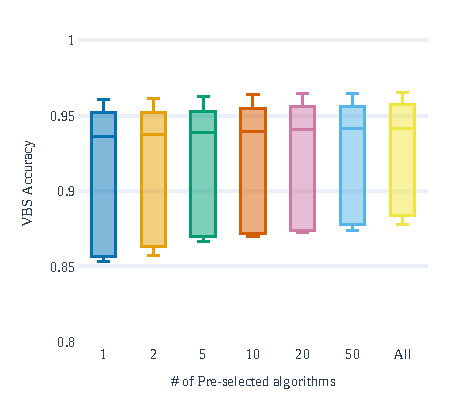
\includegraphics{figures/10/figures/analysis/zap_preselection_vbs_box.pdf}
  \caption[ZAP pre-selection quality]{ZAP pre-selection quality. 

  Each box reports held-out \gls{vbs} accuracy, after marginal-contribution pre-selection was fitted on the corresponding training fold; higher is better.}
  \label{fig:ch10:zap_preselection_vbs}
    \end{center}

\end{wrapfigure}

\cref{fig:ch10:zap_preselection_vbs} shows the \gls{vbs} accuracy achieved using different portfolio sizes, compared to using all 525 configurations. Much of the \gls{vbs} performance is retained even by small portfolios.



\cref{fig:ch10:zap_accuracy_runtime} compares selector quality and training cost. JointRankingSubsample achieves the highest mean accuracy, while SimpleRanking is very close in accuracy while being the fastest, requiring only 0.28 seconds per fold on average. PairwiseClassifier, PairwiseRegressor, and PerformanceModel also achieve competitive accuracy with training times of only a few seconds per fold. The full JointRanking model from~\citet{OztEtAl22} is slower in this experiment, requiring about 1246 GPU seconds per fold while reaching 0.869 mean accuracy. 


We can see that selector-based pre-selection turns the original large configuration space into a compact portfolio on which simple \gls{asf} selectors are competitive and substantially cheaper to train.


Notably, pre-selection not only reduces training cost but also \emph{improves} selector accuracy: JointRankingSubsample achieves 0.912 mean accuracy compared to 0.869 for the full-set JointRanking model, suggesting that the large candidate space introduces noise that hampers learning. The finding that SimpleRanking matches the accuracy of the neural JointRankingSubsample model at a fraction of the cost indicates that, for this meta-feature space, simple tabular methods with proper pre-selection suffice.


\begin{figure*}[]
  \centering
  \begin{subfigure}[t]{0.49\textwidth}
    \centering
    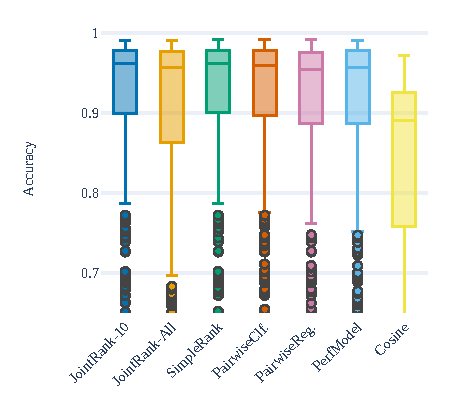
\includegraphics{figures/10/figures/analysis/zap_accuracy_box.pdf}
    \caption{Accuracy}
  \end{subfigure}
  \hfill
  \begin{subfigure}[t]{0.49\textwidth}
    \centering
    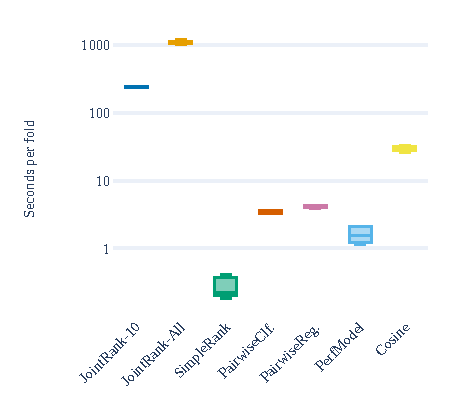
\includegraphics{figures/10/figures/analysis/zap_runtime_box.pdf}
    \caption{Running time}
  \end{subfigure}
  \caption[ZAP selector comparison]{ZAP selector comparison. The left panel reports per-dataset accuracy distributions and the right panel reports per-fold training time in seconds on a logarithmic scale. Higher accuracy and lower running time are better.



  }
  \label{fig:ch10:zap_accuracy_runtime}
\end{figure*}



\subsection{Algorithm selection for OOD generalisation}
\label{sec:ch10:ood}

Deep learning models are prone to failure when the distribution of the test data differs from the training data (known as distribution shift; see, \emph{e.g.}, \citet{WilEtAl22}). \Gls{ood} generalisation aims to train models that are robust to such shifts.

However, there exist numerous methods for the task, each specialising in different types of distribution-shift settings.
The \gls{ood}-Chameleon framework~\citep{JiaTen25} introduced algorithm selection for \gls{ood} generalisation in vision and language tasks, proposing a novel feature set that captures properties such as training-label imbalance.
The authors showed that algorithm selection can achieve state-of-the-art results, surpassing all single algorithms.

While \citet{JiaTen25} introduced algorithm selection to \gls{ood} generalisation, they did not compare against well-known algorithm selection methods and instead used an \gls{mlp}-based multi-label classifier.

We therefore investigate whether established algorithm selection methods, as implemented in \gls{asf}, can improve upon their results.


\subsubsection{Setup of experiments}
We used the \gls{ood}-Chameleon meta-dataset~\citep{JiaTen25}, which provides dataset features and algorithm performance values. We followed the original evaluation protocol for the cross-domain and in-domain transfer settings: CelebA~\citep{LiuEtAl15}/MetaShift~\citep{LiaZou22} for vision and CivilComments~\citep{BorEtAl19}/MultiNLI~\citep{WilEtAl18} for language. The base model backbones, which are the architectures to which \gls{ood} generalisation was applied, were pre-trained \gls{clip}~\citep{RadEtAl21}/ResNet~\citep{HeEtAl16}, \gls{bert}, and fine-tuned \gls{bert} (\gls{bertft})~\citep{DevEtAl19}. Cross-domain transfer means that the meta-learning tasks are sampled from different source datasets, whereas in-domain transfer means that the training and evaluation tasks are disjoint tasks sampled from the same source dataset.




\textbf{Compared selectors.} We compared the \gls{mlp} multi-label classifier from \gls{ood}-Chameleon with PairwiseClassifier, PairwiseRegressor, and PerformanceModel selectors from \gls{asf}, using random forests as the underlying machine learning models for the \gls{asf} selectors. 


\textbf{Performance metric.} As a target metric we used worst-group test error, which measures the largest error over predefined subgroups. This metric, where lower values indicate better performance, is standard in \gls{ood} generalisation, because a model can have strong average performance while still failing on minority or shifted groups. All reported results are averages over five pseudo-random number seeds.


\subsubsection{Results}
\cref{tab:ch10:ood_selector_by_scenario} reports the mean worst-group error for each training/evaluation/model combination. PairwiseRegressor turned out to be the best selector overall, with PairwiseClassifier and PerformanceModel often close. The \gls{mlp} baseline from \gls{ood}-Chameleon remains competitive, especially on several cross-dataset transfer settings, indicating that selector behaviour depends strongly on the distribution-shift structure.



The results show that pairwise regression and classification perform best in in-domain settings (same train and evaluation dataset), where the algorithm performance landscape is well-captured by the training features, while their advantage narrows in cross-domain transfer settings, where the feature distribution shifts between training and evaluation. This suggests that future work on transfer-robust features could further improve algorithm selection for \gls{ood} generalisation. 

Importantly, \gls{asf} enables this systematic comparison with minimal implementation effort: the same selector classes used for the ZAP experiment above are applied here with a different performance metric and feature set. At least one \gls{asf} selector improved over the \gls{ood}-Chameleon \gls{mlp} baseline in six of the eight training/evaluation/model combinations, including all four in-domain settings. For the other two settings, \gls{asf} selectors are on-par with the \gls{mlp} baseline. 





\begin{table*}[t]
  \centering
    \caption[OOD-Chameleon selector matrix]{\gls{ood}-Chameleon selector matrix. Rows represent training/evaluation/model combinations, columns correspond to selectors, and cells report mean worst-group error $\pm$ standard deviation over the five seeds, in percentage points. Lower is better; bold entries mark the lowest value in a row or values within 0.5 percentage points of it.

    }
  \label{tab:ch10:ood_selector_by_scenario}
  \resizebox{\textwidth}{!}{\scriptsize
\begin{tabular}{lllcccc}
\toprule
Train Data & Eval Data & Model & MLP & PairwiseClassifier & PairwiseRegressor & PerformanceModel \\
\midrule
CelebA & CelebA & CLIP & 38.6 $\pm$ 0.1 & \textbf{37.0 $\pm$ 0.1} & \textbf{37.1 $\pm$ 0.0} & \textbf{37.2 $\pm$ 0.1} \\
CelebA & CelebA & ResNet & 47.5 $\pm$ 0.1 & \textbf{45.8 $\pm$ 0.1} & \textbf{45.9 $\pm$ 0.1} & \textbf{46.0 $\pm$ 0.1} \\
CelebA & MetaShift & CLIP & \textbf{27.4 $\pm$ 0.1} & \textbf{27.5 $\pm$ 0.1} & \textbf{27.2 $\pm$ 0.3} & 28.1 $\pm$ 0.1 \\
CelebA & MetaShift & ResNet & \textbf{39.3 $\pm$ 0.2} & \textbf{39.5 $\pm$ 0.2} & \textbf{39.5 $\pm$ 0.1} & 40.1 $\pm$ 0.2 \\
CivilComments & CivilComments & BERT & 56.1 $\pm$ 0.0 & \textbf{54.8 $\pm$ 0.1} & \textbf{54.9 $\pm$ 0.1} & \textbf{55.0 $\pm$ 0.1} \\
CivilComments & CivilComments & BERT-FT & 20.9 $\pm$ 0.0 & \textbf{19.8 $\pm$ 0.1} & \textbf{19.8 $\pm$ 0.1} & \textbf{19.9 $\pm$ 0.0} \\
CivilComments & MultiNLI & BERT & \textbf{58.9 $\pm$ 0.6} & \textbf{59.2 $\pm$ 0.2} & \textbf{59.2 $\pm$ 0.3} & 59.7 $\pm$ 0.5 \\
CivilComments & MultiNLI & BERT-FT & \textbf{56.9 $\pm$ 0.2} & 57.9 $\pm$ 0.6 & \textbf{57.1 $\pm$ 0.1} & \textbf{57.3 $\pm$ 0.2} \\
\bottomrule
\end{tabular}
}

\end{table*}

\subsection{Portfolio pre-selection}


For a given task, multiple machine learning algorithms exist, each with its own hyperparameters that must be tuned.
Pre-selecting a small set of algorithm--configuration pairs that perform well across many datasets has two important use cases.
First, such portfolios can initialise hyperparameter optimisation procedures, letting the optimiser exploit known good regions instead of exploring from scratch.
Second, \gls{automl} systems such as AutoGluon~\citep{EriEtAl20} rely on pre-selected portfolios to build ensemble predictions without performing hyperparameter optimisation on the fly; selecting these portfolios well is therefore an impactful task.

However, brute-force enumeration is infeasible as the candidate set grows: there are $\binom{n}{k}$ possible subsets for $n$ candidates and portfolio size $k$ 

Therefore, efficient search algorithms are required to solve the problem.
In this section, we benchmark several such methods implemented in \gls{asf}.


\subsubsection{Setup of experiments}

We use HPOBench~\citep{EggEtAl21}, which provides performance data for traditional machine learning algorithms on OpenML datasets~\citep{BisEtAl21}. Each candidate algorithm is an algorithm-hyperparameter-configuration pair, and each pre-selector constructs a compact portfolio before being evaluated on the held-out dataset.


\textbf{Evaluation protocol.} We used leave-one-dataset-out evaluation. For each held-out dataset and portfolio size $k\in\{5,10,25\}$, the pre-selector was fitted only on the remaining datasets, and the selected portfolio was evaluated on the held-out dataset. We compared \gls{sbs} pre-selection, marginal-contribution pre-selection, beam search, random local search, genetic search, and differential-evolution-based optimisation.

\textbf{Performance metric.} Portfolio error is the minimum loss achieved by any configuration in the selected portfolio; lower is better. For visualisation, we report the normalised pre-selection \gls{sbs}-\gls{vbs} gap closed by the selected portfolio, where the performance of a portfolio on a dataset is defined by the lowest loss on the dataset of any configuration in the portfolio (\emph{i.e.}, we measure how good the selected portfolio compared to the portfolio consisting of all configurations). In this metric, 0 corresponds to \gls{sbs} and 1 corresponds to \gls{vbs}; higher is better. We also report pre-selector running time in seconds.


\subsubsection{Results}
\begin{figure*}[t]
  \centering
  \begin{subfigure}[t]{0.32\textwidth}
    \centering
    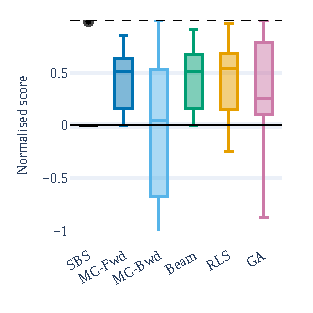
\includegraphics{figures/10/figures/analysis/hpobench_normalized_score_box_k5.pdf}
    \caption{$k=5$}
  \end{subfigure}

  \begin{subfigure}[t]{0.32\textwidth}
    \centering
    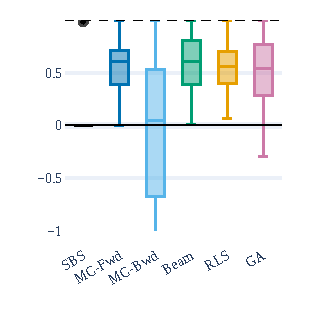
\includegraphics{figures/10/figures/analysis/hpobench_normalized_score_box_k10.pdf}
    \caption{$k=10$}
  \end{subfigure}

  \begin{subfigure}[t]{0.32\textwidth}
    \centering
    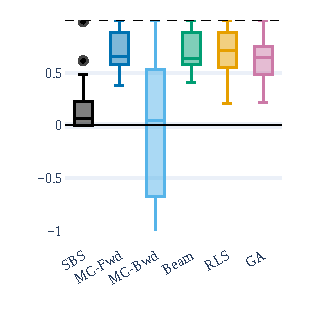
\includegraphics{figures/10/figures/analysis/hpobench_normalized_score_box_k25.pdf}
    \caption{$k=25$}
  \end{subfigure}
\par\medskip
  \begin{subfigure}[t]{0.32\textwidth}
    \centering
    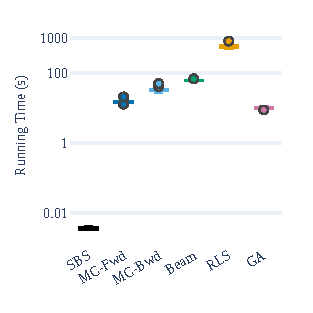
\includegraphics{figures/10/figures/analysis/hpobench_runtime_box_k5.pdf}
    \caption{$k=5$}
  \end{subfigure}
  \begin{subfigure}[t]{0.32\textwidth}
    \centering
    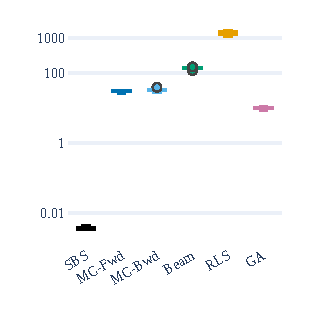
\includegraphics{figures/10/figures/analysis/hpobench_runtime_box_k10.pdf}
    \caption{$k=10$}
  \end{subfigure}
  \begin{subfigure}[t]{0.32\textwidth}
    \centering
    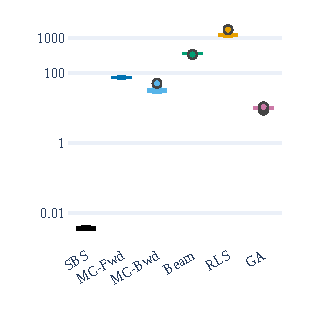
\includegraphics{figures/10/figures/analysis/hpobench_runtime_box_k25.pdf}
    \caption{$k=25$}
  \end{subfigure}
  \caption[HPOBench portfolio pre-selection by size]{HPOBench portfolio pre-selection by portfolio size. The top row reports normalised pre-selection score over held-out datasets, where 0 corresponds to \gls{sbs} and 1 corresponds to \gls{vbs}; higher is better. The bottom row reports pre-selector running time in seconds on a logarithmic scale; lower is better.}
  \label{fig:ch10:hpobench_normalized_score_box}
\end{figure*}


\cref{fig:ch10:hpobench_normalized_score_box} reports normalised pre-selection score in the top row and pre-selector running time in the bottom row. Overall, marginal contribution with forward selection, beam search, and random local search are the strongest methods. Their median scores are close across all portfolio sizes: random local search is strongest for $k=5$ and $k=25$, while beam search and forward marginal contribution are tied for the highest median at $k=10$. Genetic algorithm improves with larger portfolios but remains slightly behind these methods. Backward marginal contribution is much weaker and exhibits large negative outliers, while \gls{sbs}-based pre-selection perform closely to the \gls{sbs} (gap closed close to 0) for $k=5,10$. The overall score distributions also improve from $k=5$ to $k=25$, indicating that larger complementary portfolios close more of the gap to the \gls{vbs}. We note that differential evolution resulted in out-of-memory errors.

The methods with similar portfolio quality have different computational costs. \Gls{sbs} and marginal-contribution methods are very fast, BeamSearch is moderately more expensive, and random local search is the most expensive method. All evaluated pre-selectors run within about 1\,700 seconds on a single CPU core.




\section{Additional background}\label{sec:ch10:add_background}
Here, we provide additional background on algorithm selection.
\subsection{Algorithm Selection Baselines}
A basic, widely used baseline for algorithm selection is the single-best-solver (\gls{sbs}), which is the algorithm that works best for the instances $\mathcal{I}$. The performance of the \gls{sbs} is defined as 
$$m(SBS_\mathcal{A}, \mathcal{I})=\min_{A\in\mathcal{A}} \sum_{I\in\mathcal{I}} m(A, I)$$
Another prominent baseline is the virtual-best-solver (\gls{vbs}), also known as an oracle selector. This baseline represents an idealised, optimal selector, \emph{i.e.}, always selecting the best algorithm, which has the performance of
$$m(VBS_\mathcal{A}, \mathcal{I})= \sum_{I\in\mathcal{I}} \min_{A\in\mathcal{A}} m(A, I)$$
We note that while in machine learning (and many other fields) the algorithms are not called ``solvers'', the algorithm selection literature adopted this terminology, because the first major successes of algorithm selection came from \gls{sat} solving. Nevertheless, the definitions above apply to any domain.

\subsection{Assessment of Algorithm Selection Methods}
For algorithm selection to be feasible, there needs to be \textit{performance complementarity}, \emph{i.e.,} a single algorithm should not dominate over all problem instances.
This is a common phenomenon for many challenging computational problems, which has been thoroughly explored for $\mathcal{NP}$-complete problems~\citep{Kotthoff16,KerEtAl19}.
A simple measure for performance complementarity is the \gls{sbs}-\gls{vbs} ratio:
$$\frac{m(SBS_\mathcal{A}, \mathcal{I})}{m(VBS_\mathcal{A}, \mathcal{I})}$$
which needs to be large enough to enable viable algorithm selection.



As algorithms commonly exhibit performance complementarity, the absolute marginal contribution quantifies the contribution of an algorithm to \gls{vbs} performance:
$$\text{amc}(A, \mathcal{I}) =  m(VBS_{\mathcal{A} \backslash A}, \mathcal{I})-m(VBS_\mathcal{A}, \mathcal{I})$$
The relative marginal contribution is then defined as:
$$\text{rmc}(A, \mathcal{I})=\frac{\text{amc}(A, \mathcal{I})}{\sum_{A\in \mathcal{A}}\text{amc}(A, \mathcal{I})}$$
The marginal contribution metric is important both for analysing algorithm selection scenarios and for constructing complementary portfolios in pre-selection methods.


To measure how much of the performance difference between the \gls{sbs} and \gls{vbs} is recovered by an algorithm selector, we use the closed-gap metric:
$$\frac{m(SBS_\mathcal{A}, \mathcal{I}) - m(S, \mathcal{I})}{m(SBS_\mathcal{A}, \mathcal{I}) - m(VBS_\mathcal{A}, \mathcal{I})}$$
Where $m(S, \mathcal{I})$ is the performance of the selector. A value of 0 corresponds to \gls{sbs} performance, a value of 1 corresponds to \gls{vbs} performance, and negative values indicate performance worse than the \gls{sbs}.

\paragraph{ASlib. } \citet{BisEtAl16} have introduced a unified benchmark for algorithm selection, which includes a unified format for algorithm runs, feature values, and all other necessary information for creating an algorithm selection pipeline. The benchmark contains more than 20 algorithm selection scenarios, most of them based on running time minimisation.
ASlib has become a standard benchmark for evaluating algorithm selection systems for such use cases; however, it is less commonly used when dealing with other performance metrics.


\section{Additional discussion}

Here, we provide additional discussion related to \gls{asf}. First, we cover the differences between \gls{asf} and LLAMA~\citep{Kotthoff13}, then we cover how \gls{asf} relates to methods submitted to the algorithm selection competitions.

\subsection{LLAMA}
\label{sec:ch10:llama}
We note that LLAMA~\citep{Kotthoff13} is an established R library that helped make algorithm selection workflows more accessible and reusable. Its design anticipated several needs that remain important today, including standardised interfaces for algorithm selection experiments. However, LLAMA implements only a few basic methods, and its dependency on R limits accessibility for machine learning practitioners, where Python is the dominant language.
Additionally, while \gls{asf} supports a wide variety of methods and pipelines, LLAMA does not support, for instance, pre-selection, which we showed can significantly improve the performance of algorithm selection methods. LLAMA focuses on relatively basic selection methods, such as pairwise classification and performance prediction, while \gls{asf} covers many more approaches, including ranking-based and neural-network-based methods.

\subsection{AutoFolio and FlexFolio}
AutoFolio~\citep{LinEtAl15} is an automatic configuration system for algorithm-selection pipelines, originally designed to configure FlexFolio, a collection of algorithm-selection methods. FlexFolio was an important tool for benchmarking algorithm selectors, but it appears to be no longer actively maintained, as its implementation targets the deprecated Python 2 ecosystem. Moreover, FlexFolio focuses primarily on the selector stage and does not provide the same modular support for preprocessing, pre-solving, pre-selection, and end-to-end pipeline construction as \gls{asf}.
A newer Python 3 version of AutoFolio exists, but it supports only a restricted set of selector types, such as pairwise regression, pairwise classification, and multi-class classification. These selectors are not exposed as independently reusable Python components in the same way as in \gls{asf}. AutoFolio also supports pre-solving through Aspeed, but does not support portfolio pre-selection. Finally, AutoFolio and FlexFolio are primarily used through command-line interfaces based on the ASlib format, whereas \gls{asf} exposes a Python \gls{api} that directly accepts feature and performance matrices, while also supporting command-line usage.
\subsection{Methods from the algorithm selection competitions}
In the past, there have been two algorithm selection competitions~\citep{LinEtAl19b}. These competitions were heavily focussed on algorithm selection problems in $\mathcal{NP}$-complete 

domains, such as \gls{sat}, MIP, and TSP, while there was only a single machine learning selection scenario.
We note that the methods evaluated in these competitions are full algorithm selection pipelines, which can be easily constructed using \gls{asf} components. In the future, we plan to add pre-defined selection pipelines to \gls{asf}, which will allow users to easily use these methods. However, as these methods were developed for $\mathcal{NP}$-complete problems, they are not directly applicable to machine learning or other types of problems. As our priority is to provide a flexible framework for algorithm selection, which is applicable to any problem domain, we focussed on implementing as many components as possible, rather than implementing a small number of narrowly focussed full pipelines.

\subsection{Broader impact}
\label{sec:ch10:imapct}
Our work introduces a problem-agnostic framework for algorithm selection, with the goal of advancing research related to automated algorithm selection. In the experiments we performed and the current use cases of algorithm selection, there exist no negative societal impacts, as they are all related to foundational solutions to problems from machine learning and \gls{ai}.

\section{Example usage of ASF}
\label{sec:ch10:asf_usage_appendix}
In \cref{lst:ch10:asf_usage} we show a simple example of how to use \gls{asf} to construct a pipeline for algorithm selection. In a few lines of code, it is possible to construct a complex algorithm selection pipeline, which can be used to solve algorithm selection problems. The example shows the structure used in the experiments above: a marginal-contribution pre-selector first reduces the candidate algorithm set, and a pairwise classifier then learns to choose among the remaining candidates from instance features.


\begin{figure*}[]
\captionsetup{type=lstlisting}
\begin{minipage}{\textwidth}
\begin{lstlisting}[
  style=asfpython,
  xleftmargin=1em,
  xrightmargin=1em,
  framexleftmargin=1em,
  framesep=6pt
]
from asf.selectors import PairwiseClassifier, SelectorPipeline
from asf.pre_selector import MarginalContributionBasedPreSelector
from sklearn.ensemble import RandomForestClassifier
from sklearn.impute import SimpleImputer

features, performance = ... # Load dataset features and algorithm performance data

# Construct a pipeline: pre-select 5 algorithms, then train a pairwise classifier
pipeline = SelectorPipeline(
        selector=PairwiseClassifier(model_class=RandomForestClassifier),
        preprocessor=SimpleImputer(),
        algorithm_pre_selector=MarginalContributionBasedPreSelector(
            n_algorithms=5
        )
    )


# Fit the pipeline and predict the best algorithm for new instances
pipeline.fit(features, performance) 
predictions = pipeline.predict(features)
\end{lstlisting}
\end{minipage}
\caption[ASF usage pseudocode]{Pseudocode illustrating the usage of \gls{asf}. A pipeline is instantiated with a pre-selector and a base model, fitted on instance features and a performance matrix, and used to predict the best algorithm for new instances.}
\label{lst:ch10:asf_usage}
\end{figure*}

\section{Methods implemented in ASF}
\label{sec:ch10:methods_implemented}

\Gls{asf} covers a wide variety of algorithm selection methods. Some return a single solver, while others produce a portfolio or schedule, allowing \gls{asf} to support both classical per-instance selection and richer budget-aware decision rules.

\subsection{Selection}
\begin{itemize}
    \item \textbf{Multi-class classifier}~\citep{Kotthoff13}: Treats algorithm selection as a standard classification problem where each instance is labelled by its best algorithm. This provides a simple model-based baseline, but ignores the magnitude of performance differences between algorithms.
    \item \textbf{Pairwise classifier}~\citep{XuEtAl12}: Reduces algorithm selection to binary classification tasks, one for each pair of algorithms. Pairwise predictions are aggregated in a tournament-style vote to select the final algorithm.
    \item \textbf{Pairwise regressor}~\citep{KerEtAl18}: Trains one regressor per algorithm pair to predict performance differences. The predicted pairwise margins are aggregated into a ranking, preserving information about how large the performance gaps are.
    \item \textbf{Performance model selector}~\citep{NudEtAl04,XuEtAl08}: Fits performance prediction models and selects the algorithm with the best predicted performance. \Gls{asf} supports per-algorithm models, multi-target prediction, and joint instance-algorithm models when algorithm features are available.
    \item \textbf{Simple ranking}: Creates instance-algorithm examples by combining instance features with algorithm features or one-hot algorithm encodings. A learning-to-rank (by default, XGBoost model that uses LambdaMART~\citep{Burges10}) predicts algorithm ranks for each instance and selects the top-ranked algorithm. This is a new method implemented in \gls{asf}.
    \item \textbf{Joint ranking}~\citep{OztEtAl22}: Uses a ranking neural network over concatenated instance and algorithm representations. It scores every algorithm for a query instance and selects the algorithm with the best predicted rank.
    \item \textbf{Dyad ranking}~\citep{TorEtAl18}: A \emph{dyad} is the joint representation of an instance--algorithm pair, formed by concatenating instance features with algorithm features. The method learns pairwise rankings over these dyads, so that preferences between algorithms are informed by the combined instance and algorithm description. This is especially useful when meaningful algorithm features are available.
    \item \textbf{Survival analysis selector}~\citep{TorEtAl20,MarEtAl25}: Models time-to-completion with random survival forests, an ensemble of decision trees that estimate the survival function, \emph{i.e.}, the probability that an algorithm's running time exceeds a given threshold. This naturally handles timeouts as censored observations, since survival analysis does not require knowing the true running time of timed-out runs. The selector can choose a single algorithm or optimise a schedule that maximises completion probability under a budget.
    \item \textbf{Collaborative filtering selector (Alors)}~\citep{MisSeb17}: Treats algorithm selection as a collaborative filtering problem, where collaborative filtering is a technique from recommender systems that predicts missing entries in a user--item matrix by learning shared latent factors. Alors factorises the instance-by-algorithm performance matrix into latent instance and algorithm factors. For new instances, a regressor predicts latent factors from features and recommends the algorithm with the best reconstructed performance.
    \item \textbf{SUNNY}~\citep{AmaEtAl14,LiuEtAl21}: Finds nearest neighbours in feature space and greedily constructs a schedule that covers those neighbours well. The implementation also supports SUNNY-AS2-style tuning of the neighbourhood size and TSunny-style tuning of the schedule length.
    \item \textbf{SATzilla}~\citep{XuEtAl08}: Builds per-algorithm empirical performance models, with support for censored running time imputation and optional instance-label conditioning, where the prediction is computed as a mixture of experts.

    \item \textbf{ISAC}~\citep{KadEtAl10}: Clusters instances in feature space and assigns each cluster the algorithm with the best training performance inside that cluster. Prediction is fast because a new instance is assigned to a cluster and inherits its best algorithm, with a global-best fallback for outliers.
    \item \textbf{ISA}~\citep{LinEtAl16}: Finds similar training instances with $k$-nearest neighbours and then runs Aspeed on the neighbourhood to compute an instance-specific schedule. It is designed for running time scenarios where the output can be a schedule rather than a single algorithm.
    \item \textbf{SNNAP}~\citep{ColEtAl13}: Trains per-algorithm regressors on row-wise normalised performance and compares instances by Jaccard distance over predicted top algorithms. The selected algorithm is chosen from the best algorithms of the most similar neighbours.
    \item \textbf{Optimistic superset loss linear selector (OSLlinear)}~\citep{HanEtAl21}: Learns per-algorithm linear running time models with an optimistic superset loss for censored observations. It is intended for running time settings where timeouts provide partial rather than exact performance information.
    \item \textbf{CSHC}~\citep{MalEtAl13}: Uses a primary selector together with guardian models that estimate whether the primary choice is reliable. If confidence is too low, the method switches to a backup selector.
    \item \textbf{Cosine selector}~\citep{WuEtAl24}: Learns neural embeddings for instances and algorithms and uses cosine similarity as part of the matching model. The implementation is algorithm-feature-aware and follows the \gls{as}-LLM-style idea of fusing learned and provided algorithm representations.
    \item \textbf{Automatic parallel portfolio selector (APPS)}~\citep{KasKot23}: Trains ensembles of performance models to estimate running time distributions and uncertainty. It selects a parallel portfolio by including algorithms whose predicted distributions sufficiently overlap with the predicted best algorithm.
    \item \textbf{HARRIS}~\citep{FehEtAl22}: Builds hybrid decision-tree ensembles that combine regression loss with ranking loss based on Spearman correlation. The hybrid objective aims to predict useful performance values while preserving the relative ordering of algorithms.
    \item \textbf{Ranking by pairwise comparison (RPC)}~\citep{HulFur04}: Decomposes label ranking into binary pairwise preference problems and aggregates wins using Copeland-style scores. It can return a single algorithm or a top-$n$ parallel portfolio.
    \item \textbf{Meta-selector}~\citep{TorEtAl23}: Uses out-of-fold predictions to measure the performance of several base selectors and trains a meta-selector to choose among them. This treats selector choice itself as an algorithm selection problem.
    \item \textbf{Bagging selector}~\citep{TorEtAl23}: Trains an ensemble of selectors on bootstrap-style resamples and aggregates their predictions. This reduces variance and can make unstable base selectors more robust.
    \item \textbf{Voting selector}~\citep{TorEtAl23}: Combines several selectors by voting over their recommended algorithms. It provides a simple ensemble mechanism when multiple selectors are plausible.
    \item \textbf{Stacking selector}~\citep{TorEtAl23}: Uses predictions from base selectors as features for a meta-level selector. This allows the framework to learn how to combine heterogeneous selectors from data.
\end{itemize}

\subsection{Pre-selection}
\begin{itemize}
    \item \textbf{Marginal-contribution pre-selection}~\citep{XuEtAl08}: Selects algorithms according to their contribution to the portfolio objective. \Gls{asf} supports both backward removal from the full set and greedy forward construction.
    \item \textbf{Optimization-based pre-selection}: Treats portfolio construction as a continuous or combinatorial optimisation problem over algorithm subsets. The implementation can use differential evolution or other SciPy optimisers. This is a new method implemented in \gls{asf}.
    \item \textbf{\gls{sbs} pre-selection}: Selects the top algorithms by single-algorithm aggregate performance. This is a fast baseline that does not explicitly model complementarity.
    \item \textbf{Brute-force pre-selection}: Enumerates candidate subsets and returns the subset with the best objective value. It is exact for small candidate sets, but becomes infeasible as the number of algorithms grows.
    \item \textbf{Beam-search pre-selection}~\citep{BacEtAl22}: Builds portfolios incrementally while retaining only the best partial subsets at each step. This trades exactness for a controllable search width.
    \item \textbf{Knee-of-the-curve pre-selection}: Evaluates portfolios of different sizes and chooses the point where additional algorithms provide diminishing returns. It is useful when the desired portfolio size is not known in advance. This is a new method implemented in \gls{asf}.
    \item \textbf{Random-local-search pre-selection}: Starts from random portfolios and iteratively improves them through local changes. It provides a scalable heuristic for large algorithm sets. This is a new method implemented in \gls{asf}.
    \item \textbf{Genetic-algorithm pre-selection}: Evolves a population of candidate portfolios using mutation, crossover, and selection. This gives a flexible global-search heuristic for portfolio construction. This is a new method implemented in \gls{asf}.
\end{itemize}

\subsection{Pre-solving}
\begin{itemize}
    \item \textbf{Aspeed}~\citep{HooEtAl12}: Computes a pre-solving schedule using answer-set programming. The schedule allocates a fixed pre-solving budget across algorithms to solve easy instances before full selection.
    \item \textbf{ASAPv2}~\citep{GonEtAl17}: Optimises a preschedule over selected algorithms and time allocations. \Gls{asf} implements this as a differential-evolution-based presolver.
    \item \textbf{3S}~\citep{KadEtAl11}: Constructs a static pre-solving schedule inspired by the 3S approach. It is designed to solve many easy instances before invoking more expensive feature-based selection.
    \item \textbf{Greedy presolver}~\citep{XuEtAl08}: Builds a pre-solving schedule greedily by adding algorithm-time choices that improve the schedule objective. This is a simple and fast schedule-construction heuristic.
    \item \textbf{Configurable pre-solver}: Represents the pre-solving schedule as a configurable set of algorithm-use and time-allocation decisions. This makes pre-solving schedules amenable to external hyperparameter optimisation.
    \item \textbf{Submodular presolver}~\citep{StrGol08}: Constructs schedules using a submodular-style objective over solved instances and allocated time. It is intended to exploit diminishing returns in pre-solving coverage.
\end{itemize}

\subsection{Performance prediction}
\begin{itemize}
    \item \textbf{Empirical performance model (\gls{epm})}: Wraps a regression model with feature preprocessing, target normalization, optional imputation, and inverse transformation. It is used directly for performance prediction and internally by several selectors.
    \item \textbf{\gls{epm} tuning}: Tunes empirical-performance-model hyperparameters and target transformations by validation performance. This supports scenario-specific performance predictors for selectors such as SATzilla and performance-model selection.
\end{itemize}


\section{ASlib benchmark}
\label{sec:ch10:aslib_appendix}

We provide a benchmark of pre-selection, pre-solving, and algorithm selection based on ASlib~\citep{BisEtAl16}. Due to the large number of existing methods and the dependency of some methods on additional information (such as algorithm features, satisfiability status, and more), we selected a representative subset of methods.


We note that we used only running time-based scenarios from ASlib, namely: SAT12-INDU, SAT20-MAIN, TSP-LION2015, QBF-2016, MIP-2016, MAXSAT19-UCMS, CSP-Minizinc-Time-2016, ASP-POTASSCO, BNSL-2016, and IPC2018.

\subsection{Pre-selection}

\paragraph{Setup of experiments.}
We evaluated portfolio pre-selectors on each ASlib scenario using the pre-defined 10-fold cross-validation. We created portfolios of requested size $k\in\{2,5,10,15,20,25,30,35,40,45,50\}$; the pre-selector was fitted only on the performance matrix of the training fold and returned $k$ solvers. The selected portfolio was then evaluated on the held-out fold by the running time of its virtual best solver. 

\textbf{Performance metric.} We report the normalised held-out pre-selection score. A score of 0 corresponds to selecting the scenario single-best solver, and a score of 1 corresponds to the full virtual-best solver over all solvers. Higher values indicate that the selected portfolio preserves more of the scenario-level oracle performance.

\paragraph{Results.}
\cref{fig:ch10:aslib_preselection_a} show the distribution of normalised held-out scores across scenarios and folds for each portfolio size. The spread is largest for small portfolios, where selecting complementary solvers is a hard task, and there is a risk of the search process getting stuck in a locally optimal portfolio. By $k=10$, several search-based methods already recover most of the full \gls{vbs} performance, and increasing $k$ further mainly reduces the differences between methods. Forward marginal contribution, beam search, random local search, and genetic algorithms are consistently competitive, whereas selecting using \gls{sbs}-based pre-selection or backward marginal contribution is less robust at small and medium portfolio sizes.

\begin{figure*}[!htbp]
  \centering
  \begin{subfigure}[t]{0.32\textwidth}
    \centering
    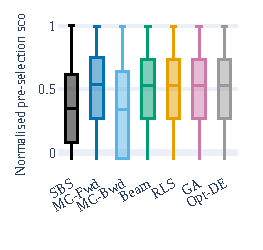
\includegraphics{figures/10/figures/analysis/preselection_normalized_score_k2.pdf}
    \caption{$k=2$}
  \end{subfigure}
  \begin{subfigure}[t]{0.32\textwidth}
    \centering
    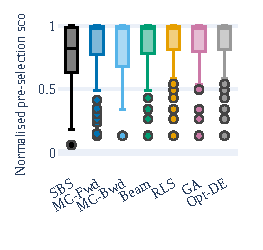
\includegraphics{figures/10/figures/analysis/preselection_normalized_score_k5.pdf}
    \caption{$k=5$}
  \end{subfigure}
  \begin{subfigure}[t]{0.32\textwidth}
    \centering
    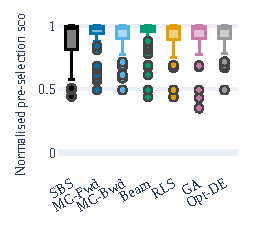
\includegraphics{figures/10/figures/analysis/preselection_normalized_score_k10.pdf}
    \caption{$k=10$}
  \end{subfigure}
  \begin{subfigure}[t]{0.32\textwidth}
    \centering
    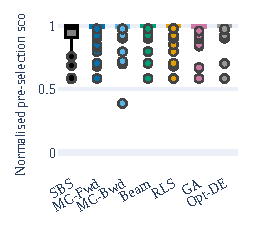
\includegraphics{figures/10/figures/analysis/preselection_normalized_score_k15.pdf}
    \caption{$k=15$}
  \end{subfigure}
  \begin{subfigure}[t]{0.32\textwidth}
    \centering
    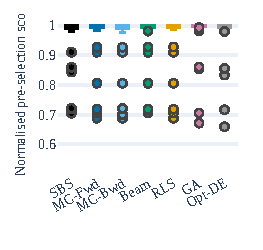
\includegraphics{figures/10/figures/analysis/preselection_normalized_score_k20.pdf}
    \caption{$k=20$}
  \end{subfigure}
  \begin{subfigure}[t]{0.32\textwidth}
    \centering
    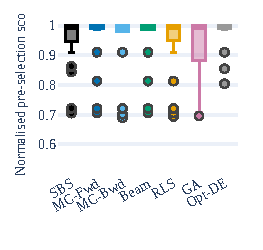
\includegraphics{figures/10/figures/analysis/preselection_normalized_score_k25.pdf}
    \caption{$k=25$}
  \end{subfigure}
  \begin{subfigure}[t]{0.32\textwidth}
    \centering
    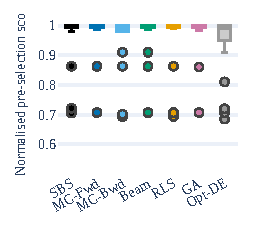
\includegraphics{figures/10/figures/analysis/preselection_normalized_score_k30.pdf}
    \caption{$k=30$}
  \end{subfigure}
  \begin{subfigure}[t]{0.32\textwidth}
    \centering
    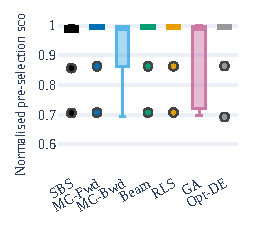
\includegraphics{figures/10/figures/analysis/preselection_normalized_score_k35.pdf}
    \caption{$k=35$}
  \end{subfigure}
  \begin{subfigure}[t]{0.32\textwidth}
    \centering
    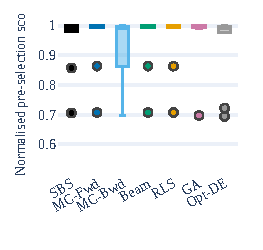
\includegraphics{figures/10/figures/analysis/preselection_normalized_score_k40.pdf}
    \caption{$k=40$}
  \end{subfigure}
  \begin{subfigure}[t]{0.32\textwidth}
    \centering
    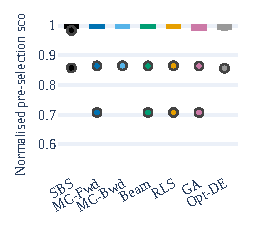
\includegraphics{figures/10/figures/analysis/preselection_normalized_score_k45.pdf}
    \caption{$k=45$}
  \end{subfigure}
  \begin{subfigure}[t]{0.32\textwidth}
    \centering
    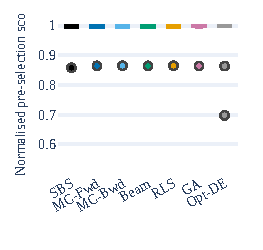
\includegraphics{figures/10/figures/analysis/preselection_normalized_score_k50.pdf}
    \caption{$k=50$}
  \end{subfigure}
  \caption[ASlib pre-selection quality by portfolio size]{ASlib pre-selection quality by portfolio size. Each box summarizes normalised held-out pre-selection score over folds and scenarios; higher is better.}
  \label{fig:ch10:aslib_preselection_a}
\end{figure*}

\clearpage

\subsection{Pre-solving}

\paragraph{Setup of experiments.}
We evaluated schedule-based presolvers on the same ASlib running time scenarios and predefined folds. For each pre-solving budget in $\{10,20,30,50,100\}$ seconds, each method was used to construct an ordered schedule of solver/time allocations on the training fold. The schedule was then tested on each held-out instance.

\paragraph{Performance metric.} We report the number of held-out instances solved within the pre-solving budget. Higher counts are better. 

\paragraph{Results.}
\cref{tab:ch10:aslib_presolving_counts} reports solved-instance counts for every scenario, budget, and presolver. 3S is the best method across most scenarios and budgets; when it is not the best, it solves only a few instances less than the best method. 

\begin{table*}[!htbp]
  \centering
  \caption[ASlib pre-solving solved-instance counts]{ASlib pre-solving solved-instance counts. Rows are grouped by pre-solving budget and ASlib scenario; columns are pre-solving methods. Higher is better, and bold entries mark the highest count in each row.}

  {\scriptsize
\setlength{\tabcolsep}{3pt}
\begin{tabular}{clccccc}
\toprule
Budget (s) & Scenario & \shortstack{ASAPv2} & \shortstack{Aspeed} & \shortstack{Greedy} & \shortstack{Static3S} & \shortstack{Submodular} \\
\midrule
\multirow{10}{*}{10} & ASP-POTASSCO & 657 & 660 & 773 & 773 & \textbf{780} \\
 & BNSL-2016 & 407 & 394 & 431 & \textbf{498} & 478 \\
 & CSP-Minizinc-Time-2016 & 49 & 51 & 57 & 56 & \textbf{61} \\
 & IPC2018 & 36 & 42 & 46 & \textbf{50} & \textbf{50} \\
 & MAXSAT19-UCMS & 153 & 150 & 209 & \textbf{210} & 186 \\
 & MIP-2016 & 51 & 43 & \textbf{73} & \textbf{73} & 60 \\
 & QBF-2016 & 584 & 591 & 543 & \textbf{616} & 608 \\
 & SAT12-INDU & 199 & 186 & \textbf{291} & 286 & 237 \\
 & SAT20-MAIN & 19 & 25 & 27 & \textbf{28} & 22 \\
 & TSP-LION2015 & 7360 & 6280 & \textbf{13170} & \textbf{13170} & 8460 \\
\midrule
\multirow{10}{*}{20} & ASP-POTASSCO & 657 & 742 & \textbf{881} & 878 & 832 \\
 & BNSL-2016 & 408 & 481 & 577 & \textbf{604} & 549 \\
 & CSP-Minizinc-Time-2016 & 49 & 58 & \textbf{62} & 61 & 61 \\
 & IPC2018 & 36 & 45 & 58 & \textbf{61} & 56 \\
 & MAXSAT19-UCMS & 153 & 181 & 225 & \textbf{249} & 213 \\
 & MIP-2016 & 51 & 52 & 84 & \textbf{93} & 77 \\
 & QBF-2016 & 585 & 609 & 618 & \textbf{626} & 624 \\
 & SAT12-INDU & 200 & 243 & 327 & \textbf{373} & 321 \\
 & SAT20-MAIN & 19 & 30 & 34 & \textbf{42} & 32 \\
 & TSP-LION2015 & 7360 & 10240 & 15070 & \textbf{18130} & 13340 \\
\midrule
\multirow{10}{*}{30} & ASP-POTASSCO & 657 & 777 & 892 & \textbf{934} & 882 \\
 & BNSL-2016 & 408 & 515 & 599 & \textbf{663} & 610 \\
 & CSP-Minizinc-Time-2016 & 49 & 58 & 61 & \textbf{62} & \textbf{62} \\
 & IPC2018 & 36 & 48 & 62 & \textbf{69} & 59 \\
 & MAXSAT19-UCMS & 153 & 190 & 240 & \textbf{276} & 247 \\
 & MIP-2016 & 51 & 59 & 84 & \textbf{99} & 84 \\
 & QBF-2016 & 588 & 608 & 642 & \textbf{647} & 636 \\
 & SAT12-INDU & 200 & 285 & 345 & \textbf{432} & 335 \\
 & SAT20-MAIN & 19 & 31 & 34 & \textbf{48} & 37 \\
 & TSP-LION2015 & 7360 & 10350 & 15650 & \textbf{20300} & 15150 \\
\midrule
\multirow{10}{*}{50} & ASP-POTASSCO & 657 & 847 & 892 & \textbf{968} & 942 \\
 & BNSL-2016 & 408 & 566 & 599 & \textbf{710} & 664 \\
 & CSP-Minizinc-Time-2016 & 49 & 59 & 61 & 64 & \textbf{65} \\
 & IPC2018 & 36 & 53 & 62 & \textbf{78} & 72 \\
 & MAXSAT19-UCMS & 153 & 202 & 240 & \textbf{302} & 277 \\
 & MIP-2016 & 51 & 63 & 84 & \textbf{114} & 98 \\
 & QBF-2016 & 588 & 630 & 642 & \textbf{675} & 636 \\
 & SAT12-INDU & 200 & 317 & 345 & \textbf{496} & 413 \\
 & SAT20-MAIN & 19 & 35 & 34 & \textbf{61} & 45 \\
 & TSP-LION2015 & 7360 & 11930 & 15650 & \textbf{24690} & 19000 \\
\midrule
\multirow{10}{*}{100} & ASP-POTASSCO & 763 & 922 & 892 & \textbf{1036} & 957 \\
 & BNSL-2016 & 495 & 677 & 599 & \textbf{826} & 683 \\
 & CSP-Minizinc-Time-2016 & 58 & 61 & 61 & \textbf{68} & 65 \\
 & IPC2018 & 49 & 65 & 62 & \textbf{104} & 71 \\
 & MAXSAT19-UCMS & 206 & 260 & 240 & \textbf{341} & 288 \\
 & MIP-2016 & 68 & 72 & 84 & \textbf{137} & 105 \\
 & QBF-2016 & 605 & 641 & 642 & \textbf{695} & 636 \\
 & SAT12-INDU & 272 & 366 & 345 & \textbf{610} & 414 \\
 & SAT20-MAIN & 25 & 46 & 34 & \textbf{76} & 46 \\
 & TSP-LION2015 & 13000 & 12920 & 15650 & \textbf{27330} & 22490 \\
\bottomrule
\end{tabular}
}
  \label{tab:ch10:aslib_presolving_counts}
\end{table*}

\clearpage

\subsection{Algorithm selection}

\paragraph{Setup of experiments. }
We evaluated learned per-instance selectors on the ASlib scenarios with predefined folds. Every learned selector first received the same fold-local forward marginal-contribution pre-selection step, retaining at most 10 solvers from the training fold. The selector was then tuned using SMAC for 50 trials using 10-fold cross-validation on the training fold and evaluated once on the held-out ASlib fold. The selector set consists of PerformanceModel~\citep{XuEtAl08}, MultiClassClassifier, PairwiseClassifier~\citep{XuEtAl12}, PairwiseRegressor, SimpleRanking, HARRIS, ISAC~\citep{KadEtAl10}, SNNAP, SUNNY, and OSLLinearSelector.

\paragraph{Performance metric.} We report the percentage of the \gls{sbs}--\gls{vbs} gap closed. A value of 0 matches \gls{sbs} and 100 matches \gls{vbs}. Negative displayed values were clipped at $-100\%$ for readability.

\paragraph{Results.}
\cref{fig:ch10:aslib_selection_gap_a,fig:ch10:aslib_selection_gap_b,fig:ch10:aslib_selection_gap_c} show that for each scenario, a different selector works well. PairwiseClassifier, PairwiseRegressor, SimpleRanking, and SNNAP are frequently among the stronger selectors, but the best method varies by scenario. For BNSL-2016 and TSP-LION2015 several selectors close a large fraction of the gap, while MIP-2016 and SAT20-MAIN remain more difficult, with all selectors solving only small fractions of the gap. MultiClassClassifier is competitive on some scenarios but less stable overall, supporting the observation made in \cref{sec:ch10:experiments} that methods exploiting pairwise or ranking information are often better suited for selection than plain multi-class classification.


\begin{figure*}[!htbp]
  \centering
  \begin{subfigure}[t]{0.98\textwidth}
    \centering
    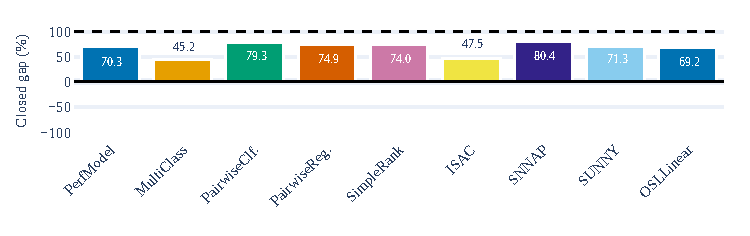
\includegraphics{figures/10/figures/analysis/selection_closed_gap_asp_potassco.pdf}
    \caption{ASP-POTASSCO}
  \end{subfigure}
  \begin{subfigure}[t]{0.98\textwidth}
    \centering
    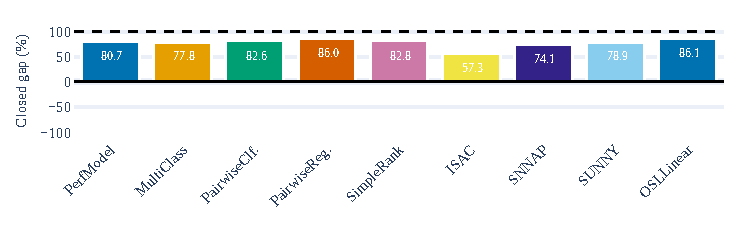
\includegraphics{figures/10/figures/analysis/selection_closed_gap_bnsl_2016.pdf}
    \caption{BNSL-2016}
  \end{subfigure}
  \begin{subfigure}[t]{0.98\textwidth}
    \centering
    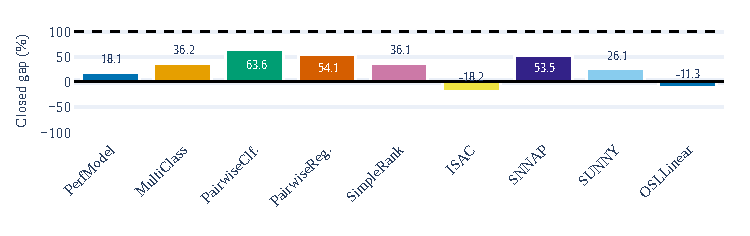
\includegraphics{figures/10/figures/analysis/selection_closed_gap_csp_minizinc_time_2016.pdf}
    \caption{CSP-Minizinc-Time-2016}
  \end{subfigure}
  \begin{subfigure}[t]{0.98\textwidth}
    \centering
    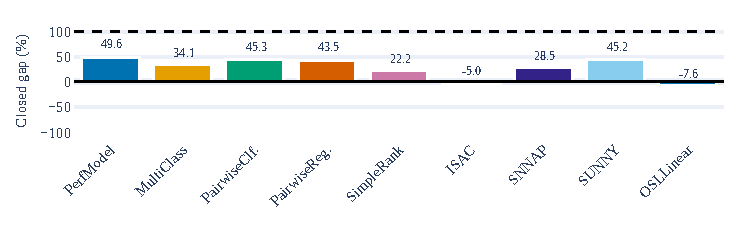
\includegraphics{figures/10/figures/analysis/selection_closed_gap_ipc2018.pdf}
    \caption{IPC2018}
  \end{subfigure}
  \caption[ASlib closed gap by scenario, part 1]{ASlib algorithm-selection closed gap by scenario and selector, part 1. Bars show the percentage of the \gls{sbs}--\gls{vbs} gap closed by each selector; higher is better. Negative displayed values are clipped at $-100\%$.}
  \label{fig:ch10:aslib_selection_gap_a}
\end{figure*}

\begin{figure*}[!htbp]
  \centering
  \begin{subfigure}[t]{0.98\textwidth}
    \centering
    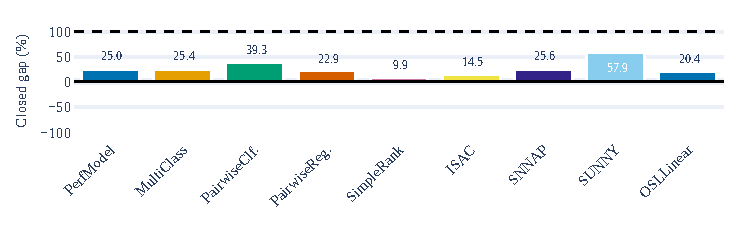
\includegraphics{figures/10/figures/analysis/selection_closed_gap_maxsat19_ucms.pdf}
    \caption{MAXSAT19-UCMS}
  \end{subfigure}
  \begin{subfigure}[t]{0.98\textwidth}
    \centering
    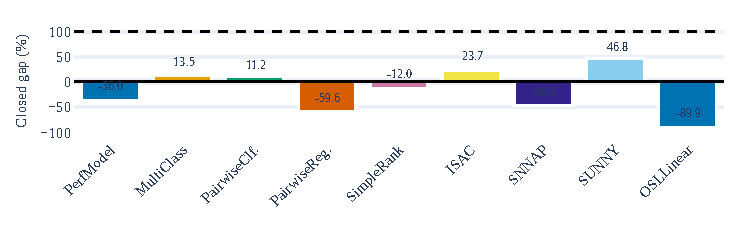
\includegraphics{figures/10/figures/analysis/selection_closed_gap_mip_2016.pdf}
    \caption{MIP-2016}
  \end{subfigure}
  \begin{subfigure}[t]{0.98\textwidth}
    \centering
    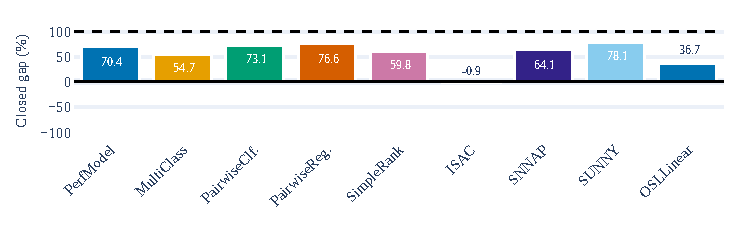
\includegraphics{figures/10/figures/analysis/selection_closed_gap_qbf_2016.pdf}
    \caption{QBF-2016}
  \end{subfigure}
  \begin{subfigure}[t]{0.98\textwidth}
    \centering
    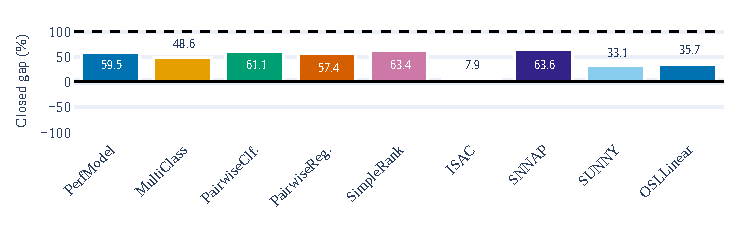
\includegraphics{figures/10/figures/analysis/selection_closed_gap_sat12_indu.pdf}
    \caption{SAT12-INDU}
  \end{subfigure}
  \caption[ASlib closed gap by scenario, part 2]{ASlib algorithm-selection closed gap by scenario and selector, part 2. Bars show the percentage of the \gls{sbs}--\gls{vbs} gap closed by each selector; higher is better. Negative displayed values are clipped at $-100\%$.}
  \label{fig:ch10:aslib_selection_gap_b}
\end{figure*}

\begin{figure*}[!htbp]
  \centering
  \begin{subfigure}[t]{0.98\textwidth}
    \centering
    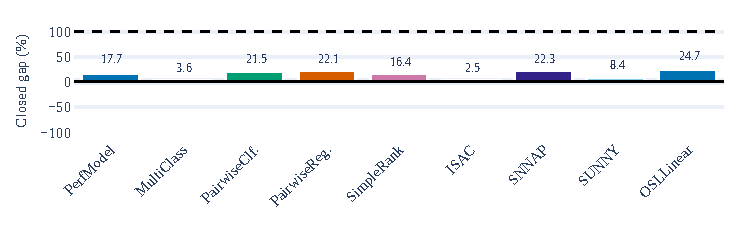
\includegraphics{figures/10/figures/analysis/selection_closed_gap_sat20_main.pdf}
    \caption{SAT20-MAIN}
  \end{subfigure}
  \begin{subfigure}[t]{0.98\textwidth}
    \centering
    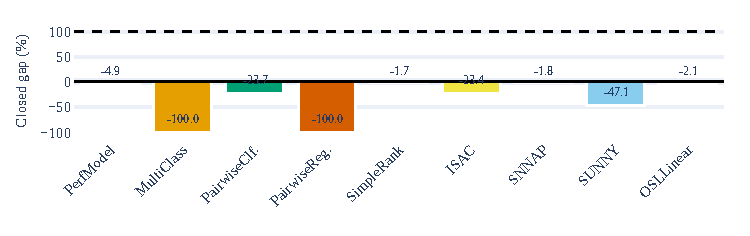
\includegraphics{figures/10/figures/analysis/selection_closed_gap_tsp_lion2015.pdf}
    \caption{TSP-LION2015}
  \end{subfigure}
  \caption[ASlib closed gap by scenario, part 3]{ASlib algorithm-selection closed gap by scenario and selector, part 3. Bars show the percentage of the \gls{sbs}--\gls{vbs} gap closed by each selector; higher is better. Negative displayed values are clipped at $-100\%$.}
  \label{fig:ch10:aslib_selection_gap_c}
\end{figure*}



\section{Additional details about the setup of experiments}
\label{sec:ch10:additional_experiment_details}

\paragraph{Hardware and launcher setup.}
Experiments were executed on a compute cluster where each CPU node is equipped with two Intel Xeon 8468 Sapphire Rapids processors, providing 96 CPU cores per node, with 256, 512, or 1024 GB main-memory configurations. The GPU nodes use the same CPU, 512 GB main memory, and four NVIDIA H100 GPUs with 96 GB HBM2e each.
We used Python version 3.10.8, clingo version 5.8.0, SMAC3 version 2.3.1, scikit-learn version 1.7.2, PyTorch version 2.9.0, XGBoost version 3.2.0. The hardware details per experiment are shown in~\cref{tab:ch10:experiment_hardware}. Additionally, the ZAP experiment used 1 H100 GPU.

\begin{table*}[!htbp]
  \centering
  \caption[Compute resources]{Compute resources used for the experiments}
  \label{tab:ch10:experiment_hardware}
  \begin{tabular}{lll}
    \toprule
    Experiment &  CPUs per task & Memory allocated \\
    \midrule
    ASlib pre-selection & 1 & 2540 MB \\
    ASlib pre-solving & 1 & 2540 MB \\
    ASlib selectors & 1 & 2540 MB \\
    HPOBench & 1 & 2540 MB \\
    \Gls{ood}-Chameleon & 1 & 5210 MB  \\
    AMLB selectors &  1 & 5210 MB \\
    ZAP selectors  & 24 & 124800 MB \\
    \bottomrule
  \end{tabular}
\end{table*}

\paragraph{Hyperparameter settings.}
We present the hyperparameter settings used in our experiments in~\cref{tab:ch10:zap_hyperparameters} to \cref{tab:ch10:aslib_presolving_hyperparameters}.
The ASlib selector benchmark tunes learned selectors with SMAC for 50 trials using 10-fold cross-validation on the training fold (\emph{i.e.}, there is an outer cross validation used for evaluation and inner cross validation for tuning, as done by~\citealp{LinEtAl15}). The tuning objective is the running-time closed gap. Before tuning each learned selector. The configuration spaces are presented in~\cref{tab:ch10:shared_configuration_spaces,tab:ch10:selector_configuration_spaces}.

\begin{table*}[!htbp]
  \centering
  \caption[ZAP experiment hyperparameters]{Hyperparameters used in the ZAP selector experiment. For JointRanking, these are the hyperparameters used by~\citep{OztEtAl22} in their code base. Since PairwiseClassifier, PairwiseRegressor, PerformanceModel and SimpleRanking have only the hyperparameters of XGBoost, we listed only them.}
  \label{tab:ch10:zap_hyperparameters}
  \scriptsize
  \begin{subtable}[t]{0.48\textwidth}
    \centering
    \caption{JointRanking}
    \begin{tabular}{ll}
      \toprule
      Hyperparameter & Value \\
      \midrule
      Epochs & 400 \\
      Batch size & 48 \\
      Learning rate & $3.018{\times}10^{-6}$\\
      Weight decay & $7.7150{\times}10^{-6}$ \\
      Hidden sizes, dropout & $(383,383,383)$ \\
      Dropout & 0.1\\
      \bottomrule
    \end{tabular}
    
  \end{subtable}
  \hfill
  \begin{subtable}[t]{0.48\textwidth}
    \centering
    \caption{JointRankingSubsample}
    \begin{tabular}{ll}
      \toprule
      Hyperparameter & Value \\
      \midrule
      Epochs & 400 \\
      Batch size & 1024 \\
      Learning rate  & $10^{-3}$ \\
      Weight decay & $10^{-5}$ \\
      Hidden sizes & $(256,256,256)$ \\
      Dropout & 0.1 \\
      \bottomrule
    \end{tabular}
    
  \end{subtable}
\hfill
  \begin{subtable}[t]{0.48\textwidth}
    \centering
    \caption{XGBoost}
    \begin{tabular}{ll}
      \toprule
      Hyperparameter & Value \\
      \midrule
      Predictor & XGBoost classifier \\
      Use weights & false \\
      \# Trees & 2000 estimators \\
      Max depth  & 6 \\
      Min child weight & 1 \\
      Learning rate & 0.3 \\
      Colsample tree / level & 1.0 / 1.0 \\
      $\lambda$, $\alpha$ & 1, 0 \\
      \bottomrule
    \end{tabular}
    
  \end{subtable}
    \hfill
  \begin{subtable}[t]{0.48\textwidth}
    \centering
    \caption{CosineSelector}
    \begin{tabular}{ll}
      \toprule
      Hyperparameter & Value \\
      \midrule
      model & neural cosine model \\
      Epochs & 200 \\
      Embedded size & 50 \\
      \# hidden layers & 2 \\
      \bottomrule
    \end{tabular}
  \end{subtable}
\end{table*}

\begin{table*}[!htbp]
  \centering
  \caption[OOD-Chameleon experiment hyperparameters]{Hyperparameters used in the \gls{ood}-Chameleon selector experiment. Each subtable gives the settings for one selector. The \gls{asf} selectors (PairwiseClassifier, PairwiseRegressor and PerformanceModel) are based on random forest.}
  \label{tab:ch10:ood_hyperparameters}
  \begin{subtable}[t]{0.48\textwidth}
    \centering
    \caption{\gls{mlp}}
    \begin{tabular}{ll}
      \toprule
      Hyperparameter & Value \\
      \midrule
      Hidden size & 100 \\
      \# Hidden layers & 1 \\
      optimizer & Adam \\
      learning rate, & $10^{-3}$ \\
      weight decay  & $10^{-4}$ \\
      Epochs & 800 \\
      \bottomrule
    \end{tabular}
  \end{subtable}
  \hfill

  \begin{subtable}[t]{0.48\textwidth}
    \centering
    \caption{Random forest}
    \begin{tabular}{ll}
      \toprule
      Hyperparameter & Value \\
      \midrule
      Trees & 100 \\
      Max depth & None \\
      min samples split  & 2  \\
      Min samples leaf & 1 \\
      \bottomrule
    \end{tabular}
  \end{subtable}
 

\end{table*}

\begin{table*}[!htbp]
  \centering
  \caption[Pre-selection experiment parameters]{Parameters used in the HPOBench and ASlib pre-selection experiments. Each pre-selector is shown in a separate subtable. Both benchmarks use the \gls{vbs} objective on the training matrix. MarginalContribution, \gls{sbs} and beam search has no parameters}
  \label{tab:ch10:aslib_preselection_hyperparameters}

  \begin{subtable}[t]{0.48\textwidth}
    \centering
    \caption{RandomLocalSearch}
    \begin{tabular}{ll}
      \toprule
      Hyperparameter & Value \\
      \midrule
      \# Restarts &  10 \\
      \# Iterations & 100 \\
      \bottomrule
    \end{tabular}
  \end{subtable}
  \hfill
  \begin{subtable}[t]{0.48\textwidth}
    \centering
    \caption{GeneticAlgorithm}
    \begin{tabular}{ll}
      \toprule
      Hyperparameter & Value \\
      \midrule
      Population size & 50 \\
      \# Generation & 100 \\
      Crossover rate & 0.8 \\
      Mutation rate & 0.1 \\
      \bottomrule
    \end{tabular}
  \end{subtable}
  \hfill
  \begin{subtable}[t]{0.30\textwidth}
    \centering
    \caption{OptimizeDE}
    \begin{tabular}{ll}
      \toprule
      Hyperparameter & Value \\
      \midrule
      Population size & 15 \\
      Max iter & 1000\\
      Population rate & (0.5, 1.0) \\
      Recombination rate & 0.7 \\
      \bottomrule
    \end{tabular}
  \end{subtable}
\end{table*}

\begin{table*}[!htbp]
  \centering
  \caption[Pre-solving experiment parameters]{Parameters used in the ASlib pre-solving experiment. Greedy presolver has no parameters.}
  \label{tab:ch10:aslib_presolving_hyperparameters}
    \begin{subtable}[t]{0.48\textwidth}
    \centering
    \caption{Submodular schedules}
    \begin{tabular}{ll}
      \toprule
      Parameter & Value \\
      \midrule
      time grids & $(5,10,20)$ \\
      Max actions &  5 \\
      \bottomrule
    \end{tabular}
  \end{subtable}
  \hfill
  \begin{subtable}[t]{0.48\textwidth}
    \centering
    \caption{ASAPv2}
    \begin{tabular}{ll}
      \toprule
      Parameter & Value \\
      \midrule
      Runcount limit & 1000 \\
      Population & 20 \\
      Population rate & (0.5, 1.0) \\
      Recombination rate & 0.7 \\
      \bottomrule
    \end{tabular}
  \end{subtable}
  \begin{subtable}[t]{0.48\textwidth}
    \centering
    \caption{Static3S}
    \begin{tabular}{ll}
      \toprule
      Hyperparameter & Value \\
      \midrule
      Max cand. sched.  &  50 \\
      \bottomrule
    \end{tabular}
  \end{subtable}
  \hfill
  \begin{subtable}[t]{0.48\textwidth}
    \centering
    \caption{Aspeed}
    \begin{tabular}{ll}
      \toprule
      Hyperparameter & Value \\
      \midrule
      Clingo cutoff & 60 s \\
      cores & 1 \\
      \bottomrule
    \end{tabular}
  \end{subtable}
\end{table*}

\begin{table*}[!htbp]
  \centering
  \caption[Shared selector configuration spaces]{Shared configuration-space components used by selector tuning. These subspaces are reused by the selector-specific spaces in \cref{tab:ch10:selector_configuration_spaces}.}
  \label{tab:ch10:shared_configuration_spaces}
  \scriptsize
  \begin{subtable}[t]{0.48\textwidth}
    \centering
    \caption{Selector pipeline}
    \resizebox{\linewidth}{!}{
    \begin{tabular}{ll}
      \toprule
      Hyperparameter & Search space \\
      \midrule
      Use presolver & Yes/No \\
      Presolver & 3S \\
      Algorithm pre-selector & MarginalContribution (forward)\\
      \bottomrule
    \end{tabular}
    }
  \end{subtable}
  \hfill
  \begin{subtable}[t]{0.48\textwidth}
    \centering
    \caption{Feature processing}
    \resizebox{\linewidth}{!}{
    \begin{tabular}{ll}
      \toprule
      Hyperparameter & Search space \\
      \midrule
      Feature group $g$ & true/false for each ASlib feature group \\
      Max feature time & $[0,\mathrm{budget}]$ \\
      \bottomrule
    \end{tabular}
    }
  \end{subtable}

  \medskip
  \begin{subtable}[t]{0.48\textwidth}
    \centering
    \caption{RF classifier/regressor}
    \begin{tabular}{ll}
      \toprule
      Hyperparameter & Search space \\
      \midrule
      \# Trees &  $[16,128]$\\
      Min samples split & $[2,20]$ \\
      Min samples leaf & integer $[1,20]$ \\
      Max features & continuous $[0.1,1.0]$ \\
      Bootstrap & true/false \\
      \bottomrule
    \end{tabular}
  \end{subtable}
  \hfill
  \begin{subtable}[t]{0.48\textwidth}
    \centering
    \caption{XGBoost classifier/regressor/ranker}
    \begin{tabular}{ll}
      \toprule
      Hyperparameter & Search space \\
      \midrule
      \# Trees &  2000  \\
      Max depth & $[1,11]$ \\
      Min child weight & $[1,100]$  \\
      Learning rate & $[10^{-3},10^{-1}]$ \\
      Colsample tree / level & $[0,1]$ \\
      $\lambda$, $\alpha$ & $[10^{-3},10^3]$ \\
      \bottomrule
    \end{tabular}
  \end{subtable}
\end{table*}

\begin{table*}[!htbp]
  \centering
  \caption[Selector-specific configuration spaces]{Selector-specific configuration spaces. Each selector is shown in a separate subtable; model-class choices recurse into the shared model spaces in \cref{tab:ch10:shared_configuration_spaces}.}
  \label{tab:ch10:selector_configuration_spaces}
  \begin{subtable}[t]{0.48\textwidth}
    \centering
    \caption{ISAC}
    \begin{tabular}{ll}
      \toprule
      Hyperparameter & Search space \\
      \midrule
      clusterer & GMeans or KMeans \\
      KMeans clusters & $[2,20]$ \\
      \bottomrule
    \end{tabular}
  \end{subtable}

  \begin{subtable}[t]{0.48\textwidth}
    \centering
    \caption{SNNAP}
    \begin{tabular}{ll}
      \toprule
      Hyperparameter & Search space \\
      \midrule
      $k$ & $[1,50]$ \\
      top-$n$ & $[1,20]$\\
      \bottomrule
    \end{tabular}
  \end{subtable}
  \hfill
  \begin{subtable}[t]{0.48\textwidth}
    \centering
    \caption{SUNNY}
    \begin{tabular}{ll}
      \toprule
      Hyperparameter & Search space \\
      \midrule
      Use v2 & True/False; \\
      $k$ & $[1,50]$ \\
      \bottomrule
    \end{tabular}
  \end{subtable}
  \begin{subtable}[t]{0.48\textwidth}
    \centering
    \caption{OSLLinearSelector}
    \begin{tabular}{ll}
      \toprule
      Hyperparameter & Search space \\
      \midrule
      Regularisation & $[0,10]$;  \\
      optimizer & [L-BFGS-B, CG, BFGS, TNC, SLSQP] \\
      max iterations & $[100,5000]$\\
      tolerance & $[10^{-6},10^{-2}]$ \\
      \bottomrule
    \end{tabular}
  \end{subtable}

\end{table*}

\section{Licensing, availability and maintenance}
\Gls{asf} is open source and is available on (deleted for anonymous submission) with \gls{mit} licence.
The authors will continue to maintain the package with newly introduced methods. Additionally, we encourage authors of newly created algorithm selection methods to implement them initially within \gls{asf}, and to submit a pull request to contribute their implementation to \gls{asf}. The authors of \gls{asf} hereby undertake the responsibility to approve any such pull request within 3 months, as long as it adheres to the \gls{asf} code standards and structure. The authors of \gls{asf} will support authors of new algorithm selection methods in implementing their methods within \gls{asf}.

\Gls{asf} includes a \gls{ci} to ensure that all new code pushed to the library is formatted according to the \gls{pep8} guidelines using the Ruff linter. Additionally, \gls{asf} includes comprehensive PyTests, which are also required to pass for every new code added. Furthermore, there are code coverage checks, which are used to ensure that every new code is accompanied with proper tests.

The anonymous code of \gls{asf} is available at \url{https://anonymous.4open.science/r/asf-660A/README.md} and of the experiments in the paper at
\url{https://anonymous.4open.science/r/asf_paper-2A6C/}.

\section{Chapter conclusion}
\label{sec:ch10:conclusion}
This chapter presented \gls{asf}, a Python framework for automated algorithm selection that brings together methods from different research communities, such as classical selectors, pairwise and ranking-based approaches, empirical performance models, pre-selection, pre-solving, and tunable end-to-end pipelines, under a single, problem-agnostic \gls{api}.

Our experiments demonstrate the practical value of this unification and reveal several cross-cutting insights.
Firstly, \emph{pre-selection is beneficial beyond reducing computational cost}: in the ZAP experiment, reducing 525 configurations to 10 cuts training time from about 1,246 GPU seconds per fold for the full JointRanking model to 0.28--9.9 seconds per fold for the fastest pre-selected \gls{asf} selectors, an improvement of up to roughly four orders of magnitude, while also improving selector accuracy by over four percentage points because the smaller candidate set reduces noise and the chance of severe selection errors.

Secondly, \emph{pairwise and ranking methods are consistently strong}: across the use cases we studied, methods that exploit the relative ordering of algorithm performance, rather than treating selection as multi-class classification, are the best-performing selectors.

Thirdly, \emph{no single method dominates everywhere}: the best selector varies across ZAP, \gls{ood}, and ASlib, and the best pre-selection method varies with portfolio size on HPOBench, highlighting the need for a unified framework that makes it easy to evaluate multiple approaches.

These findings suggest that algorithm selection should be treated as a generic problem of designing reusable pipelines rather than as a set of loosely related tasks for specific application domains.


\Gls{asf} does not remove the need for careful scenario design: selector quality depends on informative instance features, representative performance data, and an evaluation protocol that matches the intended deployment setting. However, by standardising the algorithm selection pipeline, \gls{asf} makes it substantially easier to assess and exploit the performance complementarity between different algorithms, providing a reliable framework for empirical analysis.

In the future, we plan to extend the framework with online algorithm selection, warm-starting, and tighter integration with \gls{automl} systems, with the goal of making algorithm selection even easier to apply, compare, and reproduce across machine learning and \gls{ai}.


\paragraph{Connection to the thesis}~
This chapter addresses the practical side of empirical performance prediction: methods are most useful when they can be reused, compared, and deployed through a common interface.
ASF therefore turns the methodological ideas studied throughout the dissertation into software infrastructure for algorithm selection workflows.
Together with the preceding chapters, it completes the progression from better representations, to better predictive models, to better explanations and tools; the concluding chapter synthesises these threads.
